\chapter{Probabilité, information et entropie}

\lectureoverview{La mécanique statistique commence au point de rencontre entre les lois microscopiques et une connaissance incomplète. Nous commençons par préciser la notion de probabilité, puis nous nous demandons comment le mouvement déterministe lui-même attribue des probabilités, comment les lois de conservation partitionnent l’espace des états et pourquoi une dynamique qui préserve l’information conduit naturellement à l’entropie. Les premier et zéroième principes n’interviennent qu’une fois cette structure établie.}

\section{Pourquoi la mécanique statistique ?}

On présente parfois la mécanique statistique comme une physique ancienne. Cette description passe à côté de l’essentiel. Elle est prémoderne, moderne et restera probablement utile à toute physique postmoderne qui succédera aux théories que nous connaissons. Les modèles particuliers apparaissent et disparaissent ; la deuxième loi de la thermodynamique, elle, a maintes fois résisté à l’épreuve du temps en servant de repère. Chaque fois qu’une description proposée de la nature semble créer de l’ordre gratuitement, effacer fondamentalement de l’information ou conduire un système fermé à un état anormalement simple, la deuxième loi nous avertit qu’un élément a été omis.

Le sujet peut sembler moins fascinant qu’une particule nouvellement découverte, mais il est au moins aussi profond et bien plus général. Les gaz, les liquides, les solides, le rayonnement, les trous noirs, l’information et les champs quantiques exigent tous un raisonnement statistique. En fait, les dispositifs expérimentaux utilisés pour découvrir les particules seraient incompréhensibles sans lui. C’est pourquoi des générations de physiciens de talent ont maîtrisé la mécanique statistique, même lorsque leurs principaux travaux portaient sur d’autres sujets : cette discipline est utile, mais elle est aussi d’une beauté exceptionnelle.

Pour comprendre pourquoi elle est nécessaire, partons de l’idéal proposé par la mécanique. Un système fermé est soit l’univers entier considéré, soit un sous-système suffisamment isolé pour que son environnement n’ait pas d’influence sur lui. Si nous connaissons sa condition initiale et sa loi d’évolution, la mécanique classique permet une prédiction complète. La mécanique quantique modifie ce qu’il est possible de prédire, mais elle aussi possède un état défini avec précision et une loi qui prédit l’information maximale autorisée par la théorie.

Il existe un écart considérable entre une prédiction en principe et une compréhension utile. Une liste indiquant la position et la vitesse de chaque molécule de cette pièce serait incroyablement longue, changerait presque aussitôt et répondrait à bien peu des questions qui nous intéressent réellement. Les lois microscopiques exactes peuvent donc être parfaitement prédictives et pratiquement inutiles à la fois.

La mécanique statistique est la théorie des probabilités appliquée à cette situation physique. Elle devient nécessaire lorsque la condition initiale n’est pas connue avec une précision parfaite, lorsque la loi n’est connue qu’approximativement, lorsque le système est ouvert ou, tout simplement, lorsque le nombre de variables microscopiques est trop grand pour qu’on puisse les suivre. Rien de tout cela n’implique que les prédictions soient peu fiables. Les grands nombres rendent souvent les prédictions statistiques remarquablement précises.

Considérons une boîte de gaz isolée. Nous ne pouvons pas prédire la trajectoire de chaque molécule, mais quelques données macroscopiques nous permettent de prévoir avec précision la pression, l’énergie et de nombreuses autres grandeurs globales. Ce qui reste incertain, ce sont les fluctuations. À un instant imprévisible, une petite région peut contenir plus de molécules que la moyenne, tandis qu’une autre en contient moins. Un tel événement se situe dans la queue d’une distribution de probabilité : il est improbable, mais pas interdit. Nous pouvons calculer la fréquence à laquelle de telles fluctuations devraient se produire sans prédire l’instant où surviendra un événement particulier.

Le lancer de pièces illustre la même distinction. Sur un milliard de lancers équitables, le nombre de piles et celui de faces seront presque égaux. Une longue série de piles finira par se produire si nous lançons la pièce assez souvent, mais la théorie des probabilités en prédit la fréquence, pas le moment à l’avance. La mécanique statistique est conçue pour les systèmes dont les éléments sont trop petits, trop nombreux ou les deux.

Ce cours développera les lois ainsi que leurs applications à la matière. Le sujet gagne à être étudié à plusieurs reprises : on l’apprend, on en oublie certains aspects, puis on le réapprend en comprenant mieux quelles idées sont fondamentales. Nous commençons par l’idée qui commande tout ce qui suit.

\section{La probabilité comme langage primitif}

Le calcul des probabilités lui-même n’explique pas pourquoi la probabilité fonctionne. Une prédiction probabiliste peut échouer lors d’un essai particulier ; c’est ce que signifie qu’un résultat soit possible mais improbable. La théorie nous indique comment les exceptions se répartissent. Elle ne les élimine pas. Nous prenons donc la probabilité comme un concept primitif et énonçons les règles auxquelles elle obéit.

\subsection{États et normalisation}

Soit \(i\) l’indice d’une issue possible ou d’un état possible du système. Pour une pièce, \(i\) peut désigner pile ou face. Pour un dé, il peut prendre les valeurs de \(1\) à \(6\). Pour deux dés, une paire d’indices indique les deux faces. Nous commençons par un espace d’états fini et discret,
\begin{equation}
 i=1,\ldots,N,
\end{equation}
puis nous passerons à des espaces comportant une infinité dénombrable ou continue d’états.

Ignorer quel est l’état du système ne signifie pas que celui-ci n’en a pas. Cela signifie que nous ne savons pas lequel il occupe ; nous attribuons donc une probabilité \(p_i\) à chaque possibilité. Les règles de base sont
\begin{align}
 p_i &\geq 0, \label{eq:sm1-prob-positive}\\
 \sum_{i=1}^{N}p_i &=1. \label{eq:sm1-prob-normalization}
\end{align}
Les issues possibles sont mutuellement exclusives et exhaustives : une seule d’entre elles se produit. Les probabilités négatives n’ont pas leur place ici, et leur somme vaut un puisque l’une des issues autorisées doit se produire.

\subsection{Fréquence et loi des grands nombres}

La probabilité est reliée à l’expérience par la répétition des essais. Supposons que la même expérience soit réalisée \(N_{\mathrm{trials}}\) fois, et notons \(N(i)\) le nombre d’essais qui donnent l’issue \(i\). L’interprétation fréquentiste s’écrit alors
\begin{equation}
 p_i=
 \lim_{N_{\mathrm{trials}}\to\infty}
 \frac{N(i)}{N_{\mathrm{trials}}}.
 \label{eq:sm1-frequency}
\end{equation}
Il s’agit d’une hypothèse physique exprimée au moyen d’une limite idéale. Aucun laboratoire ne réalise une infinité d’expériences. L’affirmation est que, si le nombre d’essais est suffisamment grand, le rapport se stabilise assez près de \(p_i\) pour permettre la prédiction visée. Les échantillons finis fluctuent autour de la valeur limite.

\subsection{Moyennes}

Attribuons maintenant un nombre \(f(i)\) à chaque état. Il peut s’agir de l’énergie, de la quantité de mouvement ou de toute autre grandeur que nous souhaitons mesurer. Sa valeur moyenne est
\begin{equation}
 \langle f\rangle=\sum_i f(i)p_i.
 \label{eq:sm1-expectation}
\end{equation}
La notation par crochets est commode même en dehors de la mécanique quantique. Dans le langage des fréquences, la même moyenne s’écrit
\begin{equation}
 \langle f\rangle
 =
 \lim_{N_{\mathrm{trials}}\to\infty}
 \frac{1}{N_{\mathrm{trials}}}
 \sum_i f(i)N(i).
 \label{eq:sm1-frequency-average}
\end{equation}

Pour une pièce, définissons
\begin{equation}
 f(\mathrm{H})=+1,
 \qquad
 f(\mathrm{T})=-1.
\end{equation}
Si pile et face ont chacune une probabilité \(1/2\), alors
\begin{equation}
 \langle f\rangle
 =(+1)\frac12+(-1)\frac12=0.
\end{equation}
La moyenne n’est pas nécessairement une issue possible. La pièce ne tombe jamais sur zéro ; zéro résume la distribution de ses deux valeurs possibles.

Ce bref détour fixe le vocabulaire employé dans toute la discipline : états, probabilités, fréquences et valeurs moyennes.

\section{Trois façons d’attribuer des probabilités}

\subsection{Symétrie}

Pourquoi attribuons-nous habituellement des probabilités égales aux deux faces d’une pièce ? La première réponse est la symétrie. Retourner une pièce presque idéale échange pile et face sans modifier l’expérience. Il n’y a alors aucune raison physique de privilégier l’une ou l’autre issue. Une marque ou une imperfection réelle introduit un biais minime, mais le modèle symétrique représente bien l’expérience visée :
\begin{equation}
 p(\mathrm{H})=p(\mathrm{T})=\frac12.
\end{equation}

Le même raisonnement attribue la probabilité \(1/6\) à chaque face d’un dé symétrique. Plus généralement, les configurations reliées par une symétrie reçoivent des probabilités égales, sauf si une information supplémentaire brise cette symétrie.

\subsection{Expérience}

Un dé mal équilibré ne possède aucune symétrie qui échange ses six faces. Dans ce cas, la symétrie seule ne permet pas de répondre. On peut disposer d’un modèle mécanique plus approfondi qui prédit le biais ; en l’absence d’un tel modèle, la démarche honnête est expérimentale : lancer le dé de nombreuses fois, relever les fréquences, attendre qu’elles se stabilisent et utiliser le tableau de probabilités obtenu pour les prédictions ultérieures.

La symétrie et l’expérience ne sont pas deux définitions concurrentes. Ce sont deux sources d’information sur une distribution de probabilité. La mécanique statistique s’appuiera largement sur la symétrie, mais la dynamique fournit une troisième voie.

\subsection{La probabilité issue du mouvement déterministe}

Imaginons un objet irrégulier présentant six configurations colorées. Son état change à intervalles de temps discrets et réguliers, selon une loi d’évolution définie :
\begin{equation}
 R\longrightarrow B\longrightarrow Y\longrightarrow G
 \longrightarrow O\longrightarrow P\longrightarrow R.
 \label{eq:sm1-six-cycle}
\end{equation}
L’objet lui-même n’a pas besoin de posséder une symétrie géométrique. La loi indique simplement quelle configuration succède à une configuration donnée.

\begin{figure}[htbp]
\centering
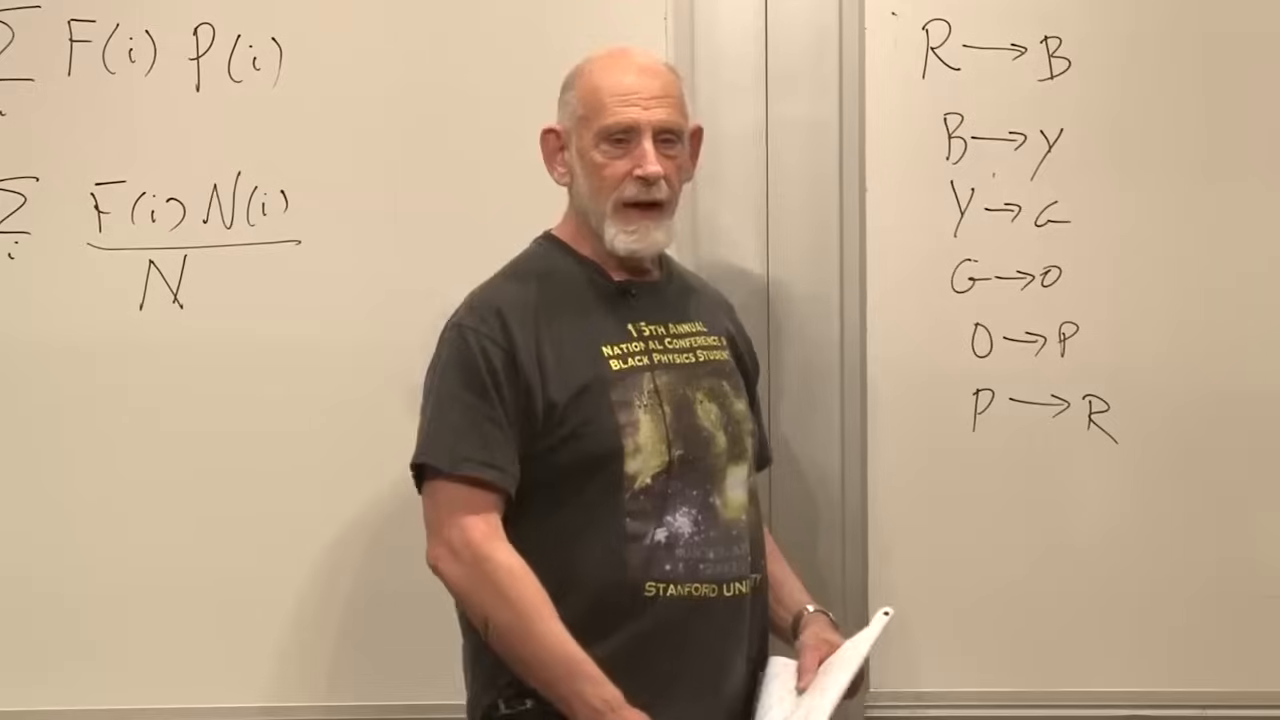
\includegraphics[width=0.92\textwidth]{lecture_01_figure_02.png}
Les formules des valeurs moyennes restent affichées sur le tableau de gauche, tandis que les six mises à jour déterministes des couleurs sont énumérées sur celui de droite.\caption{
}
\lectureframe{00:26:28}
\end{figure}

La liste au tableau se comprend mieux sous la forme d’un cycle orienté :
\begin{figure}[htbp]
\centering
\begin{tikzpicture}[
  >=Latex,
  state/.style={draw,circle,minimum size=8mm,inner sep=1pt}
]
\node[state] (R) at (90:2.2) {$R$};
\node[state] (B) at (30:2.2) {$B$};
\node[state] (Y) at (-30:2.2) {$Y$};
\node[state] (G) at (-90:2.2) {$G$};
\node[state] (O) at (-150:2.2) {$O$};
\node[state] (P) at (150:2.2) {$P$};
\draw[->] (R) -- (B);
\draw[->] (B) -- (Y);
\draw[->] (Y) -- (G);
\draw[->] (G) -- (O);
\draw[->] (O) -- (P);
\draw[->] (P) -- (R);
\end{tikzpicture}
Une orbite unique à six états. Chaque état est visité une fois par période.\caption{
}
\label{fig:sm1-six-cycle}
\end{figure}

Supposons que nous ignorions l’état initial et que nous observions le système à un instant inconnu. Chaque étape ayant la même durée, le système passe un sixième de la période dans chaque couleur :
\begin{equation}
 p(R)=p(B)=p(Y)=p(G)=p(O)=p(P)=\frac16.
 \label{eq:sm1-uniform-cycle}
\end{equation}
Cette égalité ne découle pas de la forme de l’objet. Elle vient du temps passé dans chaque état, qui est le même.

Nous pouvons réordonner les flèches et obtenir une loi microscopique différente tout en conservant un cycle unique à six états. La séquence détaillée change, mais la probabilité d’observer le système reste \(1/6\), puisque chaque état apparaît toujours une fois par période. Cette prédiction ne dépend donc ni du point de départ ni de l’ordre détaillé. Elle dépend uniquement de la structure de l’orbite et de la même durée pour chaque étape.

\begin{classroomqa}
\classquestion{Si l’objet n’est pas symétrique, en quel sens est-il
légitime d’attribuer à chaque couleur la probabilité \(1/6\) ?}
\lecturerresponse{Cette attribution découle de la dynamique, et non de la géométrie. Une observation faite à une phase inconnue d’une orbite à six étapes échantillonne six intervalles de temps égaux. L’équivalence pertinente est celle des positions sur l’orbite, et non celle des faces de l’objet. Si les durées de séjour étaient différentes, les probabilités le seraient aussi.
\lecturetimestamp{00:27:11--00:29:49}}
\end{classroomqa}

\section{Cycles disjoints et grandeurs conservées}

Une loi déterministe ne place pas nécessairement tous les états sur une seule orbite. Considérons deux cycles disjoints,
\begin{equation}
 R\longrightarrow B\longrightarrow G\longrightarrow R,
 \qquad
 P\longrightarrow Y\longrightarrow O\longrightarrow P.
 \label{eq:sm1-two-cycles}
\end{equation}
Si nous savons que le système se trouve sur le premier cycle, alors
\begin{equation}
 \begin{aligned}
 p(R)=p(B)=p(G)&=\frac13,\\
 p(P)=p(Y)=p(O)&=0.
 \end{aligned}
\end{equation}
Savoir qu’il se trouve sur le second cycle inverse ces attributions.

Le cas général nécessite des poids a priori. Étiquetons les cycles \(+1\) et
\(-1\), et notons leurs probabilités \(p_+\) et \(p_-\), avec
\begin{equation}
 p_++p_-=1.
\end{equation}
Alors
\begin{align}
 p(R)=p(B)=p(G)&=\frac{p_+}{3},\\
 p(P)=p(Y)=p(O)&=\frac{p_-}{3}.
 \label{eq:sm1-sector-weights}
\end{align}
Les facteurs \(1/3\) découlent du mouvement au sein d’un cycle. Les nombres \(p_+\)
et \(p_-\) n’en découlent pas. Ils doivent provenir d’une connaissance supplémentaire, par exemple d’une autre expérience ou d’un autre système qui sélectionne le secteur initial.

Les étiquettes \(+1\) et \(-1\) définissent une grandeur conservée : si le système commence sur un cycle, la loi d’évolution ne le transporte jamais sur l’autre. On peut appeler cette grandeur énergie ou lui donner un nom provisoire comme \emph{zilch}. Son nom importe peu. La conservation signifie que l’espace des états est partitionné en régions que la dynamique ne peut traverser.

Les cycles n’ont pas besoin de contenir le même nombre d’états. Une orbite à quatre états et une orbite à deux états définissent tout de même deux secteurs conservés. Un échantillonnage uniforme dans le temps donne alors \(1/4\) dans le premier secteur et \(1/2\) dans le second, dans chaque cas multiplié par la probabilité a priori de ce secteur. La mécanique statistique doit répondre à deux questions logiquement distinctes :
\begin{enumerate}
\item Pour un secteur conservé donné, combien de temps la dynamique passe-t-elle dans chacun de ses états ?
\item Quelle probabilité attribuer au secteur conservé lui-même ?
\end{enumerate}

\begin{classroomqa}
\audiencequestion{Supposons-nous que tous les états d’un même secteur
conservé reçoivent la même probabilité ?}
\lecturerresponse{Pour les lois discrètes simplifiées présentées ici, oui, car chaque état dure le même intervalle de temps et le mouvement est déterministe. L’incertitude porte sur la phase initiale de l’orbite. Un détecteur dont la résolution temporelle est de l’ordre de la milliseconde ne peut pas résoudre des mises à jour qui se produisent à l’échelle de la microseconde, même si un instantané suffisamment rapide peut toujours identifier l’état observé. Dans un système plus général, il faut tenir compte explicitement des durées de séjour inégales.
\lecturetimestamp{00:36:16--00:37:17}}
\end{classroomqa}

\begin{classroomqa}
\audiencequestion{Si deux instantanés sont pris et que le premier identifie un
cycle, le second devrait-il identifier le même cycle ?}
\lecturerresponse{Oui. C’est précisément ce que signifie la conservation. Une fois qu’une mesure détermine la valeur de la grandeur conservée, les probabilités futures peuvent être conditionnées par cette valeur, et la probabilité des états de l’autre secteur devient nulle.
\lecturetimestamp{00:37:18--00:37:45}}
\end{classroomqa}

\subsection{Énergie partagée entre deux systèmes}

Remplaçons maintenant l’étiquette abstraite par l’énergie. Une boîte isolée est un système fermé dont l’énergie se conserve. Deux boîtes isolées possèdent deux énergies conservées séparément, puisqu’elles n’interagissent pas. Relions-les par un passage étroit qui permet à l’énergie de circuler : les énergies individuelles peuvent alors varier, tandis que leur somme reste constante.

\begin{figure}[htbp]
\centering
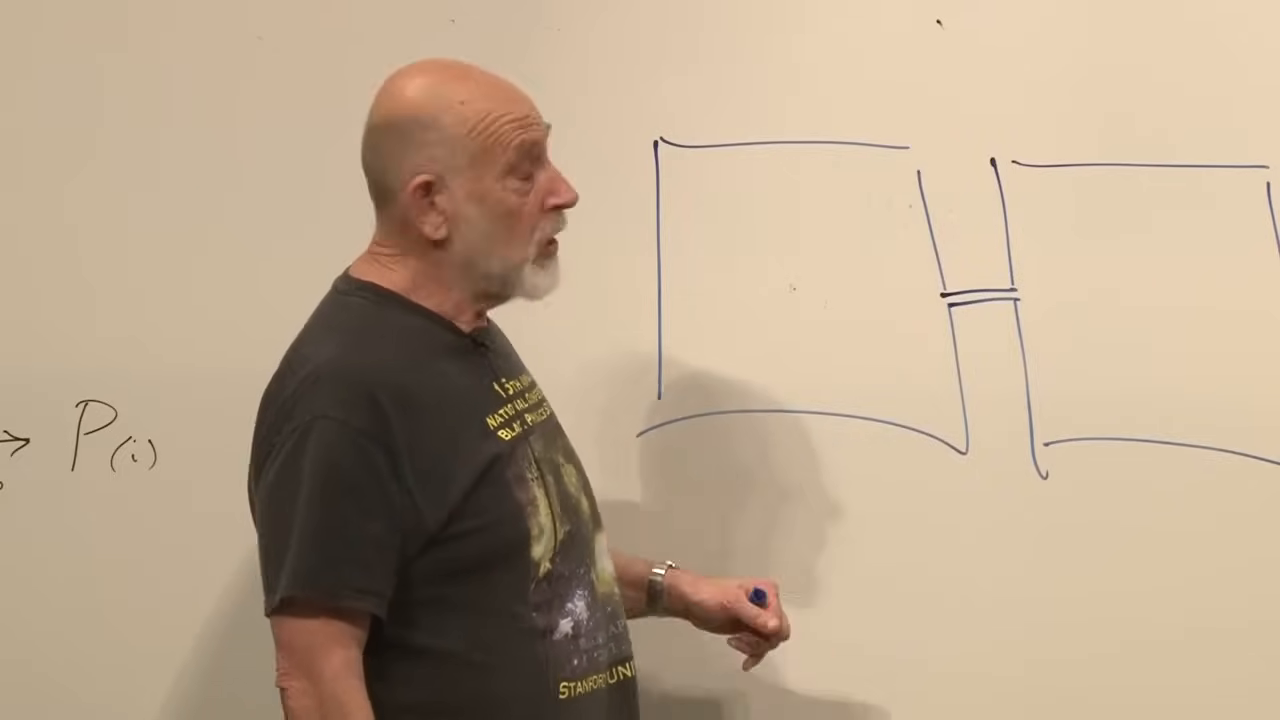
\includegraphics[width=0.92\textwidth]{lecture_01_figure_03.png}
Deux sous-systèmes reliés par un canal étroit par lequel l’énergie peut circuler.\caption{
}
\lectureframe{00:39:19}
\end{figure}

\begin{figure}[htbp]
\centering
\begin{tikzpicture}[>=Latex]
\draw[thick,rounded corners=4pt] (-4,1.8) rectangle (-0.7,-1.5);
\draw[thick,rounded corners=4pt] (0.7,1.5) rectangle (4,-1.8);
\draw[thick] (-0.7,0.45) -- (0.7,0.45);
\draw[thick] (-0.7,-0.35) -- (0.7,-0.35);
\draw[<->,very thick] (-0.45,0.05) -- (0.45,0.05);
\node at (-2.35,0.15) {subsystem \(1\)};
\node at (2.35,-0.15) {subsystem \(2\)};
\node[above] at (0,0.5) {energy exchange};
\end{tikzpicture}
\caption{Une fois la connexion établie, seule \(E_1+E_2\) est conservée.
La répartition de l’énergie devient un problème de probabilité.}
\label{fig:sm1-connected-systems}
\end{figure}

Étant donnée une énergie totale, nous pouvons demander quelle est la probabilité que le sous-système \(1\) ait une énergie \(E_1\), tandis que le sous-système \(2\) possède le reste. Des boîtes identiques devraient avoir la même énergie moyenne, mais la moyenne ne décrit pas toute la distribution. Pour déterminer les probabilités d’un sous-système, on peut donc l’inclure dans un système fermé plus grand, dont la loi de conservation fournit l’information manquante. Cette construction reviendra tout au long de la mécanique statistique.

\section{Bonnes lois, mauvaises lois et loi moins un}

Toute règle d’évolution déterministe n’est pas admissible comme loi fondamentale. Considérons l’application
\begin{equation}
 \begin{aligned}
 R&\mapsto R,& B&\mapsto R,& Y&\mapsto R,\\
 G&\mapsto R,& O&\mapsto R,& P&\mapsto R.
 \end{aligned}
 \label{eq:sm1-all-to-red}
\end{equation}
Elle prédit parfaitement l’avenir : après une étape, l’état est rouge. En revanche, elle échoue dans le sens opposé. Une fois le système à l’état rouge, rien n’indique s’il vient de l’état bleu, jaune, vert, orange ou violet, ou s’il était déjà rouge.

\begin{figure}[htbp]
\centering
\begin{tikzpicture}[
  >=Latex,
  state/.style={draw,circle,minimum size=8mm,inner sep=1pt}
]
\node[state,fill=red!12] (R) at (0,0) {$R$};
\node[state] (B) at (-3,1.6) {$B$};
\node[state] (Y) at (-3,0) {$Y$};
\node[state] (G) at (-3,-1.6) {$G$};
\node[state] (O) at (3,1.6) {$O$};
\node[state] (P) at (3,-1.6) {$P$};
\draw[->] (B) -- (R);
\draw[->] (Y) -- (R);
\draw[->] (G) -- (R);
\draw[->] (O) -- (R);
\draw[->] (P) -- (R);
\draw[->,loop above] (R) to (R);
\end{tikzpicture}
Une loi plusieurs-vers-un prédit l’état suivant, mais efface les distinctions entre les états passés possibles.\caption{
}
\label{fig:sm1-bad-law}
\end{figure}

À l’inverse, un cycle fermé préserve la trace. Si le temps écoulé est connu, nous pouvons faire évoluer l’état vers l’avenir ou vers le passé, même après plusieurs milliers de périodes. La loi préserve les distinctions entre les conditions initiales. Susskind appelle cette exigence la \emph{loi moins un de la physique} : l’information n’est pas fondamentalement perdue.

Pour un espace d’états fini et discret, le critère graphique est simple :
\begin{quote}
Chaque état d’une bonne loi possède exactement une flèche sortante et exactement une flèche entrante.
\end{quote}
La flèche sortante détermine l’avenir ; la flèche entrante permet de reconstituer le passé. Mathématiquement, la mise à jour est une permutation des états.

\subsection{Le frottement n’est qu’un contre-exemple apparent}

Le théorème de Liouville est son analogue continu. Le frottement semble le contredire. Faisons glisser une gomme sur une table : quel que soit son point de départ, elle finit par s’immobiliser. Une équation schématique de la force de frottement est
\begin{equation}
 m\ddot x=-\gamma\dot x,
 \qquad \gamma>0.
 \label{eq:sm1-drag}
\end{equation}
Sa vitesse décroît exponentiellement. Si cette équation était la loi fondamentale de chaque particule dans une pièce hermétiquement close, tout mouvement finirait par disparaître, la température tomberait à zéro et de nombreux états initiaux s’effondreraient en un seul état final. La conservation de l’énergie échouerait, l’information disparaîtrait et le désordre diminuerait. Ce serait, dans le cas continu, comme si tout finissait à l’état rouge.

Le frottement réel ne produit pas cet effet. La gomme chauffe la table, elle-même et l’environnement alentour. Les positions et quantités de mouvement microscopiques conservent la trace des distinctions perdues dans le mouvement visible. Le frottement est une équation effective pour un sous-système, obtenue après omission des degrés de liberté inobservés ; ce n’est pas une loi dissipative fondamentale décrivant le système fermé dans son ensemble.

\begin{classroomqa}
\classquestion{Que représente l’équation différentielle
\(m\ddot x=-\gamma\dot x\), et pourquoi ne peut-elle pas être une loi fondamentale
d’un système fermé ?}
\lecturerresponse{Elle représente le frottement visqueux. À elle seule, elle entraîne toutes les vitesses vers zéro, ce qui ferait refroidir un gaz jusqu’à zéro, quelle que soit sa température initiale. Dans une description réelle d’un système fermé, l’énergie mécanique et l’information perdues passent dans des degrés de liberté microscopiques. L’équation de frottement n’est fiable qu’après élimination de ces variables.
\lecturetimestamp{00:44:40--00:48:56}}
\end{classroomqa}

\section{États occupés et première entropie}

La conservation de l’information possède un équivalent probabiliste. Supposons que \(M\) états parmi \(N\) reçoivent une probabilité égale,
\begin{equation}
 p_i=
 \begin{cases}
 1/M, & i\text{ in the occupied set},\\
 0, & i\text{ outside it}.
 \end{cases}
 \label{eq:sm1-uniform-occupied}
\end{equation}
Une évolution qui préserve l’information peut redistribuer les états occupés, mais elle ne peut pas les fusionner. À tout instant ultérieur, il reste \(M\) états de probabilité \(1/M\). En revanche, la mauvaise application \eqref{eq:sm1-all-to-red} peut réduire plusieurs états occupés à un seul.

Le nombre \(M\) mesure l’ignorance. Si \(M=N\), tous les états sont possibles et notre ignorance est maximale. Si \(M=1\), l’état microscopique est connu avec exactitude. La première définition de l’entropie est donc
\begin{equation}
 S=\log M.
 \label{eq:sm1-entropy-logm}
\end{equation}
On obtient
\begin{equation}
 S_{\max}=\log N,
 \qquad
 S_{\min}=0.
\end{equation}
Si l’espace des états est infini, il n’existe pas nécessairement de borne supérieure finie.

Dans ce développement, l’entropie apparaît avant la température, et même avant l’énoncé formel de la conservation de l’énergie. En ce sens, elle est plus primitive. Pourtant, elle n’est pas une propriété du seul système mécanique. Elle dépend à la fois du système et de la distribution de probabilité qui représente ce que l’on sait. Des observateurs disposant d’informations différentes peuvent attribuer des entropies différentes au même système mécanique.

Sous l’évolution microscopique exacte, les états occupés sont simplement réarrangés ; cette entropie à grain fin se conserve donc. En pratique, nous perdons la trace du temps, négligeons les corrélations et ne suivons pas un nombre immense de variables. Notre distribution de probabilité s’étale alors sur un plus grand nombre de possibilités, et l’entropie attribuée à la description macroscopique augmente. Les équations n’ont pas besoin de détruire l’information pour que notre description exploitable en perde.

\begin{classroomqa}
\classquestion{Quelle est l’entropie maximale possible d’un système fini
comportant \(N\) états ?}
\lecturerresponse{C’est \(\log N\) ; elle est atteinte lorsque les \(N\) états sont tous équiprobables. L’entropie minimale est zéro ; elle est atteinte lorsqu’un état a une probabilité égale à un. L’entropie mesure donc à la fois l’état de nos connaissances et l’espace des états accessibles.
\lecturetimestamp{00:56:46--00:58:19}}
\end{classroomqa}

\section{Écoulement de Liouville dans l’espace des phases continu}

Pour des particules dont les positions et les quantités de mouvement sont continues, un état microscopique est un point de l’espace des phases. Nous notons les coordonnées \(q_a\) et leurs moments conjugués \(p_a\). Avec un grand nombre de particules, les axes sont extraordinairement nombreux ; un dessin en deux dimensions comportant un \(q\) et un \(p\) n’est qu’une représentation simplifiée. L’espace des phases est de dimension paire, car chaque coordonnée a un moment qui lui est associé.

Supposons que notre connaissance soit représentée par une région \(\Omega_0\) : la densité de probabilité est uniforme à l’intérieur de cette région et nulle à l’extérieur. Par exemple, savoir que chaque particule se trouve dans la pièce restreint les coordonnées de position, tandis que des bornes sur leurs vitesses restreignent les coordonnées de moment.

L’évolution hamiltonienne entraîne chaque point de l’espace des phases le long d’une trajectoire. Des points voisins restent voisins, et la région occupée s’écoule comme une parcelle de fluide incompressible :
\begin{figure}[htbp]
\centering
\begin{tikzpicture}[>=Latex,scale=0.95]
\draw[->] (-4.2,0) -- (4.3,0) node[right] {$q$};
\draw[->] (-3.7,-2.2) -- (-3.7,2.4) node[above] {$p$};
\draw[fill=blue!12,thick]
  (-3.0,-0.5) .. controls (-2.7,1.0) and (-1.3,1.2) .. (-0.9,0.1)
  .. controls (-0.6,-1.0) and (-2.2,-1.4) .. cycle;
\node at (-1.9,0.0) {$\Omega_0$};
\draw[->,very thick] (-0.3,0.2) -- (0.8,0.2);
\draw[fill=orange!15,thick]
  (1.2,-1.1) .. controls (1.5,0.3) and (2.3,1.8) .. (3.2,1.1)
  .. controls (3.6,0.7) and (2.8,-0.4) .. (2.5,-1.5)
  .. controls (2.1,-1.8) and (1.5,-1.6) .. cycle;
\node at (2.35,0.1) {$\Omega_t$};
\end{tikzpicture}
L’écoulement hamiltonien peut étirer et cisailler une région occupée de l’espace des phases, mais il en conserve le volume.\caption{
}
\label{fig:sm1-liouville-flow}
\end{figure}

Le théorème de Liouville énonce que
\begin{equation}
 \operatorname{Vol}(\Omega_t)
 =
 \operatorname{Vol}(\Omega_0).
 \label{eq:sm1-liouville-volume}
\end{equation}
Si la densité initiale est uniforme sur \(\Omega_0\), la densité transportée est uniforme sur \(\Omega_t\). C’est l’analogue continu de la conservation du nombre et des poids des états discrets occupés.

Le théorème résout aussi géométriquement le problème du frottement. Si nous ne considérons que la quantité de mouvement visible de la gomme, un nuage de possibilités semble se resserrer vers \(p=0\). Dans l’espace des phases complet, le nuage s’étale dans les positions et les quantités de mouvement des molécules de la gomme et de la table. Une projection peut se contracter tandis que le volume total de l’espace de grande dimension reste constant.

\begin{classroomqa}
\classquestion{Si toutes les trajectoires visibles tendent vers le repos, la
région occupée de l’espace des phases s’est-elle effondrée sur l’axe \(p=0\) ?}
\lecturerresponse{Uniquement dans la projection réduite. Le système complet
comprend les variables microscopiques de la table, de la gomme et de l’environnement. À mesure que l’intervalle des quantités de mouvement visibles se resserre, la distribution s’étale dans ces directions cachées. Le théorème de Liouville s’applique à l’espace des phases complet du système fermé, et non à un ensemble incomplet de variables macroscopiques.
\lecturetimestamp{01:04:37--01:06:29}}
\end{classroomqa}

\section{De la loi moins un au premier principe}

\subsection{Bref aperçu du principe zéro}

Avant d’énoncer le premier principe, il est utile de nommer le principe zéro. L’équilibre thermique n’a pas encore été défini ; pour l’instant, le principe se limite à un énoncé structurel :
\begin{quote}
Si le système \(A\) est en équilibre thermique avec \(B\), et si \(B\) est en équilibre thermique avec \(C\), alors \(A\) est en équilibre thermique avec \(C\).
\end{quote}
Cette transitivité permettra plus tard de définir la température. Pour le moment, nous la laissons de côté.

\subsection{Conservation de l’énergie}

Le premier principe pour un système fermé s’écrit simplement
\begin{equation}
 \frac{dE}{dt}=0.
 \label{eq:sm1-first-law}
\end{equation}
Cette forme concise dissimule toute sa portée. L’énergie est une grandeur conservée, et le terme « énergie » prendra plus tard un sens thermodynamique plus riche.

Si un système fermé est constitué de deux parties et que leurs énergies sont additives,
\begin{equation}
 E=E_1+E_2,
\end{equation}
alors
\begin{equation}
 \frac{dE_1}{dt}+\frac{dE_2}{dt}=0,
 \qquad\text{or}\qquad
 \frac{dE_1}{dt}=-\frac{dE_2}{dt}.
 \label{eq:sm1-energy-exchange}
\end{equation}
La seconde forme rend l’échange explicite : l’énergie perdue par un sous-système est gagnée par l’autre.

L’hypothèse d’additivité demande quelques précautions. Deux particules en interaction gravitationnelle possèdent chacune une énergie cinétique, mais leur interaction ajoute une énergie potentielle qui appartient à la paire. L’énergie totale se conserve, même si elle ne peut pas s’écrire exactement comme la somme de l’énergie de l’une et de celle de l’autre.

La thermodynamique autorise souvent une excellente approximation additive, car l’énergie globale est proportionnelle au volume, tandis que l’énergie d’interaction à courte portée entre de grands éléments voisins dépend surtout de leur aire de contact. Divisons une grande table en blocs : l’énergie interne de chaque bloc est un effet de volume, tandis que le couplage entre blocs adjacents est un effet de surface. Pour de grands blocs, ce dernier est relativement faible. L’équation
\eqref{eq:sm1-first-law} est exacte pour l’ensemble fermé ; la forme exprimée pour les sous-systèmes,
\eqref{eq:sm1-energy-exchange}, suppose que l’énergie d’interaction est négligeable.

\begin{classroomqa}
\audiencequestion{La normalisation \(\sum_i p_i=1\) suppose-t-elle aussi que
les issues énumérées sont mutuellement exclusives ?}
\lecturerresponse{Oui. L’étiquette d’un état est définie de sorte que les possibilités ne se recouvrent pas : si le dé est dans l’état jaune, il n’est pas simultanément dans l’état rouge. Dans le langage courant, on peut mélanger les couleurs, mais la partition des états utilisée dans le calcul des probabilités doit être constituée d’issues mutuellement exclusives.
\lecturetimestamp{01:12:14--01:12:55}}
\end{classroomqa}

\section{Retour à l’entropie}

Le cours revient maintenant explicitement à une question laissée en suspens. Bien que familière à nos sens, la température est une grandeur dérivée. L’entropie et l’énergie doivent être établies avant que l’on puisse définir proprement la température.

\subsection{Distributions de probabilité générales}

La définition particulière \(S=\log M\) s’applique lorsque \(M\) états sont équiprobables et que tous les autres ont une probabilité nulle. Une distribution générale n’est pas nécessairement rectangulaire. Ses poids peuvent varier de façon régulière ou irrégulière selon les étiquettes des états.

\begin{figure}[htbp]
\centering
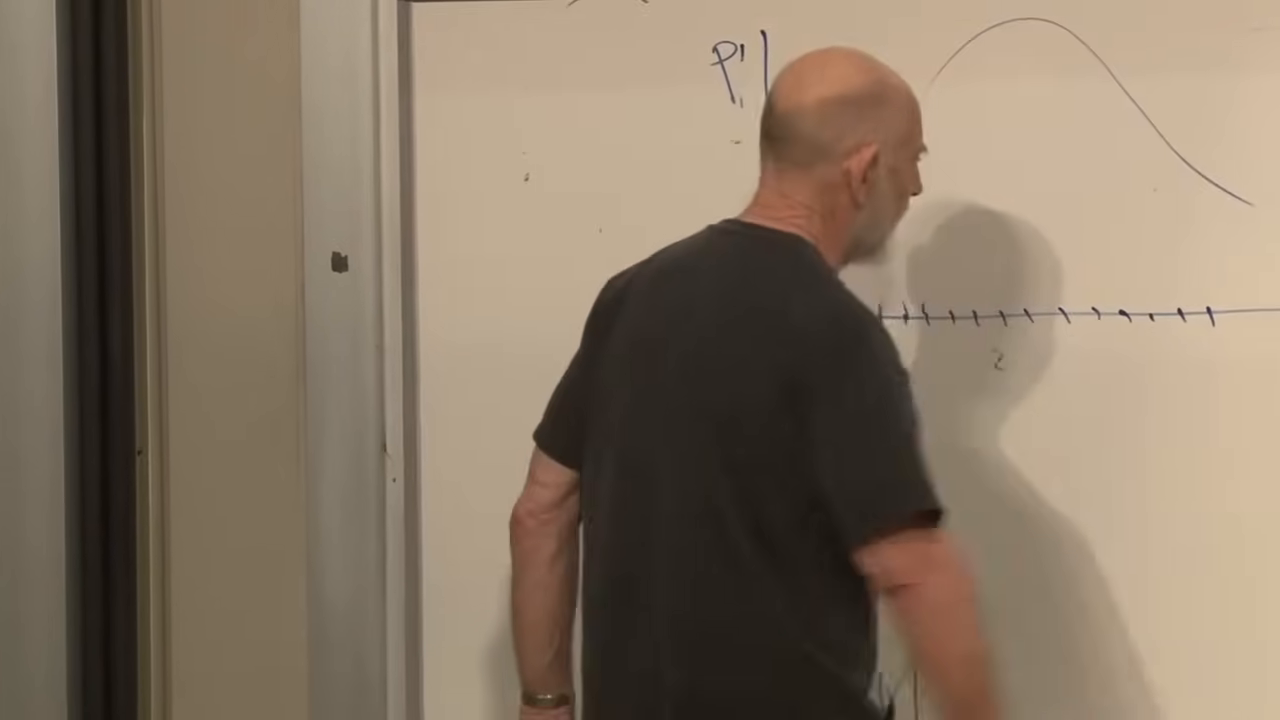
\includegraphics[width=0.92\textwidth]{lecture_01_figure_05.png}
Une distribution de probabilité représentée sur des étiquettes d’états discrètes. Pour l’entropie, c’est l’étendue, et non la courbe précise, qui importe.\caption{
}
\lectureframe{01:14:40}
\end{figure}

\begin{figure}[htbp]
\centering
\resizebox{\linewidth}{!}{%
\begin{tikzpicture}[>=Latex,scale=0.93]
\draw[->] (-4.2,0) -- (4.4,0) node[right] {state label \(i\)};
\draw[->] (-4,0) -- (-4,3.2) node[above] {$p_i$};
\foreach \x in {-3.6,-3.1,...,3.6}
  \draw (\x,0.08) -- (\x,-0.08);
\draw[very thick]
  plot[smooth] coordinates {
  (-3.7,0.12) (-3.0,0.28) (-2.3,0.72) (-1.6,1.45)
  (-0.9,2.25) (-0.2,2.65) (0.5,2.28) (1.2,1.55)
  (1.9,0.88) (2.7,0.38) (3.5,0.14)};
\draw (-1.8,-0.18) -- (-1.8,-0.5);
\draw (1.8,-0.18) -- (1.8,-0.5);
\draw[<->] (-1.8,-0.46) -- (1.8,-0.46);
\node at (0,-0.82) {effective spread};
\end{tikzpicture}
}
Une distribution étroite comporte moins d’incertitude qu’une distribution large. L’entropie doit mesurer la distribution dans son ensemble.\caption{
}
\label{fig:sm1-probability-spread}
\end{figure}

La définition générale est
\begin{equation}
 S=-\sum_i p_i\log p_i.
 \label{eq:sm1-shannon-entropy}
\end{equation}
En utilisant \eqref{eq:sm1-expectation}, on obtient
\begin{equation}
 S=-\langle\log p\rangle.
\end{equation}
Le signe moins compense le fait que \(\log p_i<0\) lorsque
\(0<p_i<1\).

\subsection{Retrouver le résultat uniforme}

Il faut vérifier que la formule générale reproduit la première définition.
Pour un état inoccupé, \(p_i=0\) alors que \(\log p_i\) diverge. Le produit
admet la limite bien définie
\begin{equation}
 \lim_{p\to0^+}p\log p=0.
 \label{eq:sm1-plogp-limit}
\end{equation}
Ainsi, les états de probabilité nulle ne contribuent pas.

\begin{classroomqa}
\audiencequestion{Si \(p_i=0\), le terme s’annule-t-il vraiment ? Le logarithme
de zéro vaut moins l’infini.}
\lecturerresponse{Le terme est défini par la limite
\(\lim_{p\to0^+}p\log p\), qui vaut zéro. Le facteur \(p\) tend vers zéro
plus rapidement que le logarithme ne diverge. Ainsi, les états arbitrairement improbables apportent des contributions arbitrairement faibles, et un état strictement impossible ne contribue pas.
\lecturetimestamp{01:18:27--01:19:46}}
\end{classroomqa}

Pour chacun des \(M\) états occupés, \(p_i=1/M\). On a donc
\begin{align}
 S
 &=-\sum_{\mathrm{occupied}\ i}
 \frac1M\log\!\left(\frac1M\right)\\
 &=-M\frac1M\log\!\left(\frac1M\right)\\
 &=-\log\!\left(\frac1M\right)
 =\log M.
 \label{eq:sm1-entropy-check}
\end{align}
L’expression générale coïncide exactement avec l’expression particulière. Une distribution plus étalée accorde un poids appréciable à davantage de possibilités et a donc une entropie plus élevée ; une distribution plus resserrée a une entropie plus faible.

\begin{figure}[htbp]
\centering
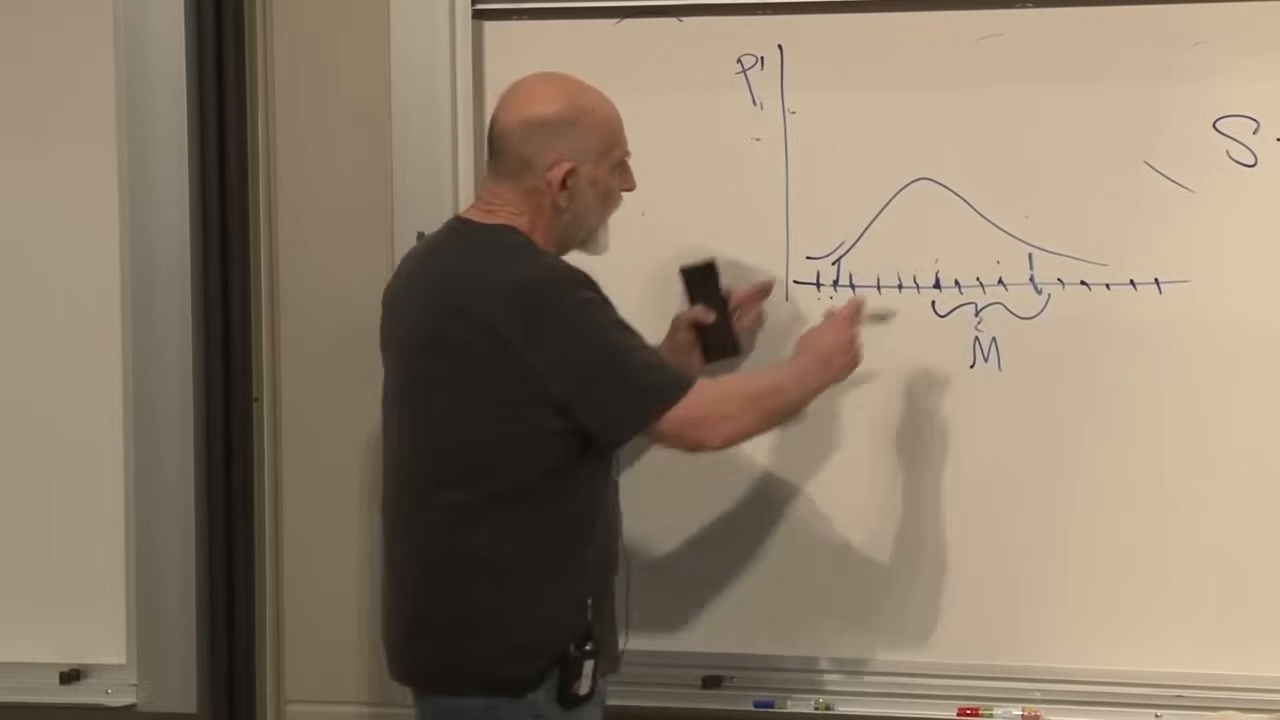
\includegraphics[width=0.92\textwidth]{lecture_01_figure_06.png}
\caption{La largeur indiquée \(M\) souligne le lien entre l’étalement des probabilités significatives et l’entropie.}
\lectureframe{01:16:42}
\end{figure}

L’entropie est associée à une distribution de probabilité sur l’espace des états. Ce n’est pas une observable prise isolément, comme l’énergie ou la quantité de mouvement d’un microétat. Un état exact peut être représenté par une distribution concentrée sur cet état ; son entropie est alors nulle. Mais l’entropie change lorsque l’état de connaissance change.

\section{Pièces, bits et dénombrement explicite}

Soit \(n\) le nombre de pièces. Le nombre de configurations microscopiques est
\begin{equation}
 N=2^n.
 \label{eq:sm1-coin-state-count}
\end{equation}
Si l’on ne sait rien des pièces, les \(2^n\) configurations sont toutes équiprobables, et
\begin{equation}
 S_{\max}=\log(2^n)=n\log2.
 \label{eq:sm1-coin-max-entropy}
\end{equation}
L’entropie est additive en fonction du nombre de pièces indépendantes.

Avec des logarithmes en base \(2\), un système à deux états totalement inconnu a une entropie d’un bit. Avec des logarithmes népériens, son entropie vaut \(\log2\). L’unité est conventionnelle ; l’ordre sous-jacent et l’additivité restent inchangés.

À l’autre extrême, si l’on connaît l’état de chaque pièce, une seule configuration a une probabilité égale à un :
\begin{equation}
 S=0.
\end{equation}
Plus on dispose d’informations, plus l’entropie est faible.

Supposons maintenant qu’exactement une des \(n\) pièces soit côté pile et que toutes les autres soient côté face, sans que l’on sache où se trouve celle qui est côté pile. Il y a \(n\) configurations équiprobables, une pour chaque position possible de cette pièce, donc
\begin{equation}
 S=\log n.
 \label{eq:sm1-one-tail-entropy}
\end{equation}
Ce n’est généralement pas un multiple entier de \(\log2\). Le bit est une unité pratique ; cela ne signifie pas que toute entropie soit un nombre entier de bits.

\begin{classroomqa}
\audiencequestion{\(\log2\) n’apparaît-il que parce que chaque pièce a deux états possibles ? Un élément à trois états donnerait-il \(\log3\) ?}
\lecturerresponse{Exactement. Un élément dont l’état est uniformément inconnu parmi \(k\) états possibles contribue \(\log k\). Les commutateurs binaires sont particulièrement pratiques dans les ordinateurs, car les commutateurs physiques réalisent naturellement deux états stables et parce que deux est le plus petit entier non trivial.
\lecturetimestamp{01:29:55--01:30:48}}
\end{classroomqa}

\begin{classroomqa}
\audiencequestion{Quelle base faut-il utiliser pour le logarithme ?}
\lecturerresponse{Dans ces formules de physique, \(\log\) désigne le logarithme népérien. Les théoriciens de l’information utilisent souvent la base \(2\) ; l’entropie est alors directement exprimée en bits. Changer de base multiplie toutes les entropies par un même facteur de conversion et ne modifie aucune conclusion physique.
\lecturetimestamp{01:30:49--01:32:06}}
\end{classroomqa}

\section{Entropie dans l’espace des phases continu}

Revenons à un espace des phases classique \(\Gamma\). Si la densité de probabilité est uniforme dans une région de volume \(V_\Gamma\) et nulle à l’extérieur, l’analogue du dénombrement de \(M\) états équiprobables est
\begin{equation}
 S=\log\!\left(\frac{V_\Gamma}{V_0}\right).
 \label{eq:sm1-continuous-uniform}
\end{equation}
Ici, \(V_\Gamma\) est le volume dans l’espace complet, de grande dimension, des coordonnées et des quantités de mouvement, et non un volume spatial ordinaire. Le volume fixe \(V_0\) est une cellule de référence de l’espace des phases qui rend le logarithme sans dimension. En posant \(V_0=1\), on obtient l’écriture abrégée \(S=\log V_\Gamma\) utilisée au tableau.

Pour une densité de probabilité générale \(P(q,p)\), la somme discrète devient une intégrale sur l’espace des phases. La normalisation s’écrit
\begin{equation}
 \int_\Gamma d\Gamma\,P(q,p)=1,
 \label{eq:sm1-continuous-normalization}
\end{equation}
et l’entropie
\begin{equation}
 S=-\int_\Gamma d\Gamma\,
 P(q,p)\log\!\bigl[P(q,p)V_0\bigr].
 \label{eq:sm1-continuous-entropy}
\end{equation}
La densité est une probabilité par cellule de l’espace des phases. Conceptuellement,
\eqref{eq:sm1-continuous-entropy} mesure toujours l’étalement de la distribution de probabilité ; pour un domaine uniforme, elle se réduit au logarithme du volume occupé, exprimé en unités de la cellule de référence. Modifier cette cellule fixe décale toutes les entropies continues d’une même constante additive et laisse inchangées leurs différences.

\begin{classroomqa}
\audiencequestion{Pourquoi le symbole de coordonnée passe-t-il de \(x\) à \(q\) ?}
\lecturerresponse{Il n’y a aucun changement physique. En mécanique classique, on utilise couramment \(x\) ou \(q\) pour les coordonnées et \(p\) pour les quantités de mouvement conjuguées. Le changement de notation n’était qu’un lapsus ; la construction de l’espace des phases reste la même.
\lecturetimestamp{01:37:10--01:37:39}}
\end{classroomqa}

La température et la distribution de Boltzmann sont volontairement abordées plus tard. La prochaine étape consistera à définir l’équilibre thermique, puis à identifier la distribution de probabilité qui lui correspond.

\section{Questions sur la corrélation, l’additivité et l’information}

\subsection{La corrélation signifie qu’une mesure modifie une autre distribution}

Lorsqu’on ignore tout de pièces indépendantes, on attribue la même probabilité à chaque configuration. Mesurer l’une des pièces n’apprend alors rien sur les autres. Leurs distributions restent inchangées.

L’ensemble à une seule pièce côté pile est différent. Si la pièce mesurée est côté pile, toutes les autres sont certainement côté face. Si la pièce mesurée est côté face, la seule pièce côté pile doit se trouver parmi les \(n-1\) restantes ; chaque position restante a donc une probabilité conditionnelle de
\begin{equation}
\begin{aligned}
 p(&\text{tail at a specified remaining position}\\
   &\mid\text{measured head})=\frac{1}{n-1}.
\end{aligned}
 \label{eq:sm1-conditional-tail}
\end{equation}
C’est cela, la corrélation : apprendre la valeur d’une variable modifie la distribution de probabilité attribuée à une autre.

\begin{classroomqa}
\audiencequestion{Dans les exemples d’entropie, a-t-on supposé que les pièces étaient indépendantes ?}
\lecturerresponse{Seulement lorsque l’ignorance complète était représentée par des probabilités égales pour les \(2^n\) configurations. Dans ce cas, mesurer une pièce ne modifie pas les distributions des autres. L’exemple à une seule pièce côté pile présente explicitement une corrélation : une mesure actualise ce qui est possible ailleurs. C’est l’information énoncée qui détermine la distribution de probabilité utilisée.
\lecturetimestamp{01:38:43--01:41:58}}
\end{classroomqa}

L’exemple des cycles disjoints a la même structure logique. Mesurer l’étiquette conservée \(+1\) ou \(-1\) restreint tous les états ultérieurs à un seul secteur. Conditionner la distribution sur l’information conservée modifie les états admissibles.

L’entropie est additive pour des systèmes non corrélés. Si
\begin{equation}
 p_{ij}=p_i^{(A)}p_j^{(B)},
\end{equation}
alors
\begin{align}
 S_{AB}
 &=-\sum_{i,j}p_i^{(A)}p_j^{(B)}
 \log\!\left[p_i^{(A)}p_j^{(B)}\right]\\
 &=S_A+S_B.
 \label{eq:sm1-entropy-additivity}
\end{align}
Les corrélations empêchent cette factorisation et réduisent l’incertitude indépendante du couple.

À titre d’exercice, considérons une rangée de variables binaires telle que, lorsqu’un site est dans l’état haut, chacun de ses voisins a une probabilité de trois quarts d’être dans l’état bas. Mesurer un site modifie immédiatement ce que l’on sait des sites voisins. Une telle distribution est corrélée ; on ne peut donc pas calculer son entropie en additionnant les entropies de chaque site pris isolément sans tenir compte de ces corrélations.

\subsection{Boltzmann, Shannon et l’incertitude quantique}

\begin{classroomqa}
\audiencequestion{Quel est le lien entre l’ancienne entropie thermodynamique et l’entropie de Shannon, issue de la théorie de l’information ?}
\lecturerresponse{La même forme fonctionnelle apparaît dans les deux cas :
\(-\sum_i p_i\log p_i\). Shannon utilisait souvent la base \(2\), tandis que les physiciens emploient généralement les logarithmes népériens et réintroduisent la constante de Boltzmann lorsque l’entropie est exprimée en unités thermodynamiques. La différence mathématique se réduit à un facteur de conversion constant, même si les questions physiques à l’origine des probabilités peuvent être très différentes.
\lecturetimestamp{01:44:05--01:46:06}}
\end{classroomqa}

Pour des microétats équiprobables, la formule thermodynamique s’écrit souvent
\begin{equation}
 S_{\mathrm{thermo}}=k_{\mathrm B}\log W,
 \label{eq:sm1-boltzmann-formula}
\end{equation}
où \(W\) est le nombre de microétats accessibles. Dans les unités où \(k_{\mathrm B}=1\), cela donne précisément \(S=\log W\). La constante de Boltzmann convertit les unités de température en unités d’énergie ; à l’échelle microscopique, la température est naturellement exprimée en énergie.

\begin{classroomqa}
\audiencequestion{Cette entropie est-elle simplement une autre forme du principe d’incertitude de Heisenberg ?}
\lecturerresponse{Non. L’entropie dont il est question ici mesure l’incertitude d’une distribution de probabilité sur les états possibles. Dans le langage quantique, elle mesure l’incertitude d’un état mixte, et non l’incertitude intrinsèque de mesure qui peut subsister même pour un état pur. Il faut distinguer ces deux notions.
\lecturetimestamp{01:46:07--01:47:31}}
\end{classroomqa}

\section{Résultats établis}

Le point de départ n’était pas le caractère aléatoire des lois. Une dynamique déterministe, combinée à une connaissance incomplète de l’état initial, suffit déjà à produire des probabilités. Une trajectoire unique attribue des poids selon le temps passé dans chaque état ; les orbites disjointes révèlent des quantités conservées et exigent des poids a priori entre les secteurs. Les lois microscopiques admissibles préservent les distinctions : dans un espace d’états fini, cela signifie qu’il y a une flèche entrante et une flèche sortante en chaque état ; en mécanique continue, cela devient le théorème de Liouville.

Cette structure conduit d’abord à
\begin{equation}
 S=\log M
\end{equation}
pour \(M\) états occupés équiprobables, puis à
\begin{equation}
 S=-\sum_i p_i\log p_i,
\end{equation}
et enfin à son intégrale sur l’espace des phases. L’entropie décrit une distribution de probabilité et, par conséquent, un état de connaissance. La loi microscopique préserve l’information à grain fin, même lorsqu’une description pratique à grain grossier cesse d’en rendre compte.

La conservation de l’énergie donne la première loi, tandis que l’additivité des énergies des sous-systèmes exige que l’énergie d’interaction soit négligeable. L’entropie est additive sous une condition analogue : les probabilités des sous-systèmes doivent être non corrélées. Ces deux formes d’additivité préparent l’étape suivante, où l’équilibre thermique, la température et la distribution de Boltzmann relieront l’énergie à la probabilité.